\section{Client Design}
\label{client_design}

This section will outline our initial design of the system. We aimed for a high degree of modularity to separate concerns among team members and improve the ease of maintaining code. The process of identifying the concerns of the client and representing these in a component based design will be discussed in subsection \ref{client_approach}. The remainder of the section will discuss our design of individual components, and how we identified their roles within the larger system. Particular focus will be made on how we made sure sections of the client were removed as far as possible from other sections, and challenges in ensuring this requirement. 

\subsection{Approach}
\label{client_approach}

In designing the client, we had the high level aim of creating a modular system to allow team members to take responsibility for certain aspects of the system. From an early stage in the design process, we were aware that the client had a large set of responsibilities. We determined these responsibilities to be: to maintain a connection with the server, implement the GIM protocol, provide a user interface to the system and keep a record of up to date information about the user's friends. Our first task was to design a set of interacting sub-components to handle these responsibilities.

It was agreed that the MVC (Model-View-Controller) architectural pattern, widely used for applications involving a graphical user interface, was a useful model to base our discussions around. This model abstracts the UI (view) from the back end of the system. When a user performs an action, the controller updates the model if any data associated with the system is changed, and updates the viewer to reflect these changes in the system state. This seemed appropriate to our needs of keeping and displaying an up-to-date record of the user's friend list and creating an interface, and would allow us to split responsibilities between the back and front end of the GUI.

However, we faced challenges in adapting an additional networking component to implement the GIM protocol into this framework. We had the choice to conceptualise it as either an additional interface, which was `controlled' by the server and controller, or indirectly (by way of the network) as a part of the controller component. As an additional interface, it could `view' changes from users on the friends list, as notified by the server, and view changes to the model that it needed to know about. Although this was an interesting conceptual idea, it was difficult to consider how, or if, it could work in practicality. We decided it could be more useful to treat the networking code as part of the controller, as it would be modifying the model based on the server's response to its requests, and modifying the GUI to reflect these changes. However, for the sake of design, it was more useful to think of it as a distinct component the controller interacted with, as this would allow us to separate the concern of networking from the rest of the client.
	
This high level approach allowed us to draw boundaries between components and assign the more detailed design of individual components to team members. We decided a logical split would be to assign two members to the networking aspects of the system (client and server), and two members to the GUI components of the system (the GUI and its model). However, further collaboration was required to allow this design to happen in parallel. This involved planning how the components would talk to one another, as will be discussed in in section \ref{controller}

\subsection {Model-Viewer-Controller}

This section will explain how we designed our model, viewer, and controller components in our client. It will also outline some of the interactions between components, as outlined in figure \ref{mvc}. 

\subsubsection {Controller}
\label{controller}

\begin{figure}
    \begin{center}
        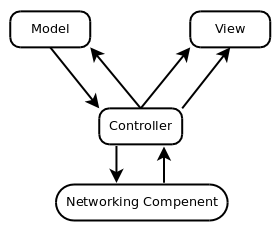
\includegraphics[scale=0.65]{Design/diagrams/mvc.png}
        \caption{The MVC pattern.}
        \label{mvc}
    \end{center}
\end{figure}

The controller was one of the more challenging parts of the design process. The controller would be called by both the networking component and the viewer, implying that its operations must be thread safe. We were constrained by our use of the Java Swing\footnote{\texttt{http://download.oracle.com/javase/6/docs/technotes/guides/swing/}} environment, which we had learned from previous experience will freeze if the networking code is run on the GUI thread. A further complexity was ensuring that the controller could use the commands of the GIM protocol without having to know its workings in detail. Naturally, the GUI architects should not need to concern themselves with the specifics of the protocol while designing the GUI.

To deal with the threading complexity, we designed a scheme with an intermediate buffer between the controller component and the networking code. The controller thread waits until there is a command from the network placed into the buffer, and acts accordingly on the model and GUI. Furthermore, when the controller component needs to call the network, it places a command into the buffer to be interpreted by the networking code. We believed this scheme to be appropriate as the controller could either call the network from internal code or events from the GUI, possibly simultaneously (See section \ref{networking_design} for further discussion on the motivation behind this buffer).

To deal with the design complexity of abstracting the protocol from the controller's use of its commands, the network architects designed two interfaces to describe the different methods. One interface contained method stubs concerning incoming commands from the server, and the other methods that could be called to send commands to the server. This allowed other team members to understand what the controller must do to implement the GIM protocol, without having to understand the inner workings of the protocol. This had the additional advantage of allowing the structure of the protocol to change, without having to change the interface or consult the team members working on other areas of the GUI. Another way we kept it unnecessary for other team members to understand the protocol was the inclusion of a parsing method in the controller the networking architects would write. This method parses incoming messages from the server and calls the appropriate method. The methods called would be written by any team member. The network architects would then be responsible for implementing the methods in the interface for outgoing commands to the server.

\begin{figure}
    \begin{center}
        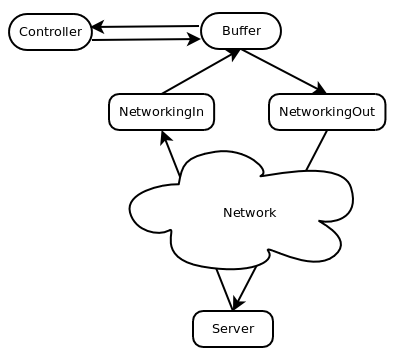
\includegraphics[scale=0.65]{Design/diagrams/buffer.png}
        \label{buffer}
    \end{center}
\end{figure}

\subsection {Model}
\label{model}

The design of the model involved determining what state information had to be held about the client. This was informed by the previous work of requirements analysis and the conception of features. The model was also informed by the design of the viewer.

Two ``must haves'' of the system were the presence of a contact list and support for user statuses. This implied that there should be data structures for these items. To deal with this requirement, we designed the model to have a data structure to maintain information about users, including their status, nickname and personal messages. 

The view required that the user's own state information (such as status and nickname) were displayed. As these were evident in multiple windows in the view design (such as in chat windows, and on the buddy list), the model was designed to maintain a record of the user's current status. 

\subsection {Viewer}

After some interface design work (see section \ref{gui_design} for more of a discussion), it was apparent that the system had to support two different styles of chat windows: a group chat and a chat with a single user. However, there were some observable commonalities between both windows, such as sending messages, displaying incoming messages, and using very similar Java Swing components to handle this functionality. At the same time, there was enough differing behaviour between the two windows to justify having two different classes to handle them, such as the group chat's need to maintain a list of users in the room. With this in mind, we designed our class structure code dealing with the interface to have a super class named ChatWindow, outlining this common functionality, which two sub classes called GroupChatWindow and SingleChatWindow which would extend this super class. 

We anticipated this would be advantageous as it would reduce the repetition of code and keep functionality consistent between the two windows. We felt this consistency would be important, as our code using the Swing components used to display messages would evolve, or need configuring, as we implemented some of our `should have' features (such as emoticons and font colours.) Therefore, this class structure would be crucial for the displaying of messages in Group Chat and SingleChat windows to remain consistent.

\begin{figure}
    \begin{center}
        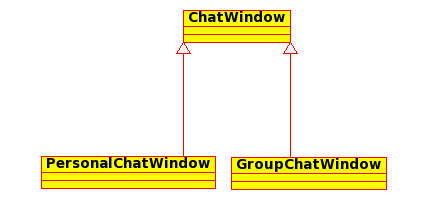
\includegraphics[scale=0.65]{Design/diagrams/chatwin.png}
        \label{chatwin}
    \end{center}
\end{figure}

\section{Design of Client GUI}
\label{gui_design}

As we had decided to incorporate both group and one-to-one chats, this provided a wide scope in terms of interface design. We had the option to base our interface on either IRC or Windows Live Messenger style clients, or to create something entirely of our own. Windows Live was ultimately selected as the basis of the GUI for a number of reasons; primarily we believed that it was better suited to our feature set. An IRC style interface would require a considerable amount of redesigning to accommodate features such as display pictures, contact lists, and offline messaging. While creating our own style of IM interface would be interesting, it would likely lead to an inferior design, and be more time consuming to create. Windows Live style programs typically integrate the vast majority--if not all--of our MoSCoW feature set (in section \ref{features}), and was therefore chosen as our starting point.

With any user interface, the primary goal is usability. As instant messengers have existed for a number of years, there is a standard layout which users expect and are comfortable with. The goal of our GUI was to provide a simple and intuitive interface, without using something too different from what users would expect from an IM application.
 
\subsection{Example Use Cases}

The GIM use cases were created in order to provide an easily understood reference for how the system should operate at a high layer of abstraction. The following are our most important use cases as defined during the design process. Two actors were identified for the system: ``Senders'' and ``Contacts.'' Both of these actors have equal privileges within the system and use the system in the same way, hence both derive from the ``User'' type. This distinction between senders and contacts is made for the design process, as in reality users of the system are both senders and contacts.

{\bf Add Contact}\\
Sender clicks the ``add contact'' button in the main window, or the option from the top menu. They are prompted to enter the contacts's email. They enter the email and the system searches for that person in the database. If found, the contacts is sent a request for friendship. If the contact accepts, then both the sender and contact now have each other as contacts, and they show up in the main window. If not accepted, neither is added. If the contact is not found, they are prompted again to enter the email, with the option to cancel.

{\bf Group Chat}\\
Sender can choose to group chat from the main window button, main menu, or in a chat window with another contact. A window will show up in which the sender can create a chatroom, and then the sender will be prompted to choose the contacts they wish to invite. The chatroom appears to the sender. Those contacts will see the invitation, and if they accept, will be placed in the chatroom. Contacts will be able to invite other people as well. The chatroom will disappear once every user has left.

{\bf Log Out}\\
User clicks the ``log out'' option in the menu. The X in the corner will only minimize the program. A dialog box appears, asking if they are sure they want to log out. If yes, they are logged out, and the log in/register pop-up appears. If they want to quit the program completely, they will have to choose``quit'' from the menu.

At this stage of the process we had begun to make a few implementation decisions, and while some aspects of each use case were ommitted in the final product, generally these specifications were adheared to. Much of the redundancy was removed, primarilly due to time restrictions. For example the number of ways to start a group chat is reduced to one, from the three ways mentioned in the use case. Group chats can only be started by pressing the button on the main window in the final program. In contrast to this, the ``Log Out'' use case is implemented to this specification exactly.

The use of informal notation for the use cases was, in retrospect, ill-conceived. A more formal notation including pre and post conditions, non-functional requirements, and priorities would have provided a better foundation for implementation. An example of where this caused confusion was in the implementation of blocking and removing contacts, where the pre and post conditions varied in subtle ways. However, due to the scope of the project and the time restrictions, we felt that these simple use cases were adequate for our needs.

\subsection{Interface Wireframes}

With these use cases we started to design a GUI that could accommodate the desired features. Although many UI sketches were made, they were all minor variations on the core design which we derived from the traditional instant messenger model, such as used in Windows Live.

\begin{figure}[!h]
    \begin{center}
        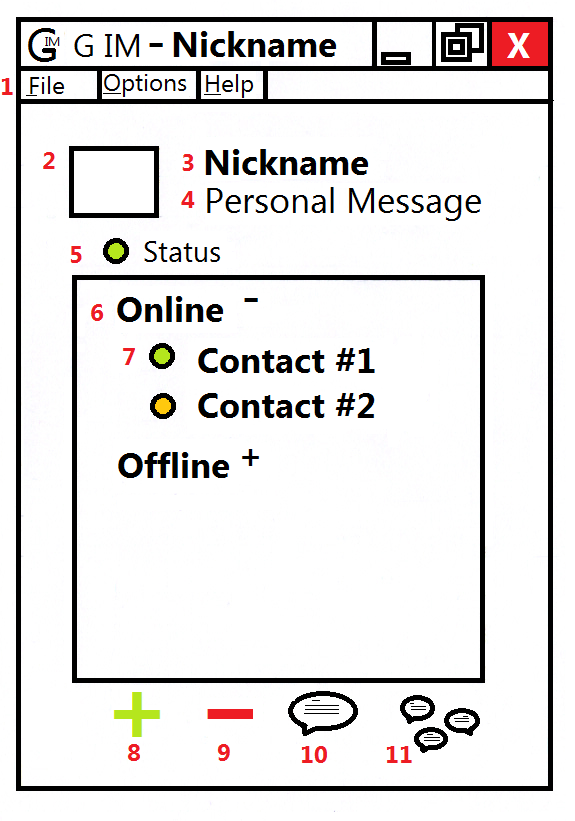
\includegraphics[width=7cm]{Design/diagrams/Main_UI.png}
        \caption{The original wireframe for the main window of the client.}
        \label{mainui}
    \end{center}
\end{figure}

{\bf Walkthrough}

\begin{enumerate}

\item Menu - Drop down menus which provide more options for the user, such logging out and qutting the program.
 
\item Display Picture - An image which represents the user. This image box also acts as a button allowing users to select a different picture.

\item Nickname - An editable text box which allows the user to change their display name. Their account name used to log in is not affected.

\item Personal Message - An editable text box which allows the user to set a message viewable by other users.

\item Status - The user can choose from a set list of statuses, which will change their icon to indicate the selected status to other users.

\item Contact List - The list of online and offline contacts the user has added to their contact list.

\item Contact - A selectable element in the contact list representing a user. Contains a display picture, username, personal message and status.

\item Add User - Brings up a prompt to input a user's email address and, if successful, adds them to the contact list.

\item Remove User - Brings up a prompt to remove the selected user from the contact list.

\item Start Chat - Creates a chat window with the selected contact.

\item Start Group Chat - Creates a group chat window with only the current user.

\end{enumerate}

The above wireframe is the main window the user will see after they have logged in. The layout is typical of instant messenger programs, and represents what users would expect to see.

\begin{figure}[!h]
    \begin{center}
        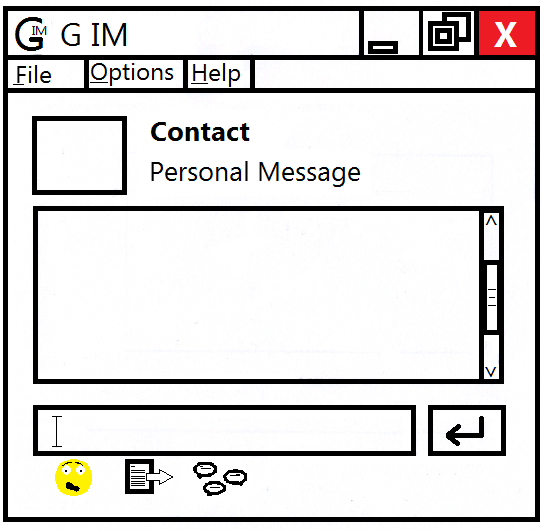
\includegraphics[width=7cm]{Design/diagrams/Chat_Box.png}
        \caption{The original wireframe design of a chat window for the client.}
        \label{chatBox}
    \end{center}
\end{figure}

This wireframe represents the window which is created when a chat is initiated, either by themselves or another user. The chat box has a similar layout to the main window, to aid consistency. The user details are at the top, the main body of content is in the middle, and the user operations are at the bottom.

These wireframes served as the basis for the Swing implementation. While the features of the final interface are unchanged from the wireframes, some slight alterations were made to the layout. These modifications were typically the result of the practicalities of using Swing and natural evolution during implementation. Examples of these alterations are the removal of buttons for emoticons, file transferring, and group chat, and a different position for the status icons in the main window. These changes are discussed in more detail in section \ref{guiimpl}.
